\documentclass[fontset=windows,a4paper,12pt]{ctexart}
\usepackage{graphicx}
\usepackage{subfigure}
\usepackage{graphics}
\usepackage{overcite}
\usepackage{CJK}

\pagestyle{plain}
\usepackage{bm}
\usepackage{amsmath}
\usepackage{multirow}

\evensidemargin 3mm \oddsidemargin 3mm
\textwidth 154mm \textheight 225mm

\begin{document}

\begin{titlepage} \begin{center} % Upper part of the page 
  \textsc{\LARGE 2016数学建模校赛}\\
  [1.5cm] \textsc{\Large 题目\quad B}\\
  [0.5cm]\ \\
  [0.4cm] { \huge \bfseries 印制电路板焊锡}\\[0.4cm]\ \\[1.5cm]\ \\[1.4cm]\ 
  \large {学\quad\quad 校:} 
  \begin{minipage}[t]{0.4\textwidth}
    \centering
    \uline{\hspace{3em}山西大学\hfill} \makebox[0.46em]{}\par
  \end{minipage}
  \\[0.6cm]
  \large {队\quad\quad 员:} 
  \begin{minipage}[t]{0.4\textwidth} 
    \uline{\hspace{3em}李恩宾 \hfill} \makebox[0.46em]{}\par
    \uline{\hspace{3em}张红若 \hfill} \makebox[0.46em]{}\par
    \uline{\hspace{3em}张彪\quad \hfill} \makebox[0.46em]{}\par
  \end{minipage}
  \\[0.6cm]
  \large {指导教师:} 
  \begin{minipage}[t]{0.4\textwidth}
    \centering
    \uline{\hspace{3em}李顺勇 \hfill} \makebox[0.46em]{}\par
  \end{minipage}
  \vfill % Bottom of the page 
  {\large \today} \end{center} \end{titlepage}
  \begin{center}
    \zihao{3}{\heiti 印制电路板焊锡}
  \end{center}
  \linespread{1.2}
  \begin{center}
    \zihao{4}{\heiti 摘\ \ \ \ 要}
  \end{center}
  \zihao{4}{\songti 
    针对电路板焊锡过程中点胶机的涂锡膏顺序问题,本文将电路板中所有的位点抽
    象为图中的顶点,将位点间的连边抽象成顶点间的连边,位点间的距离抽象为边
    上的权值,构建赋权完全图。通过遗传算法和贪婪算法,求解赋权完全图中的最
    小哈密尔顿圈,即求得最优焊锡顺序和相应的路径长度。\cite{楼建华2003数学建模与数学实验}
  }
  \\
  关键词:\ 遗传算法\ 旅行商问题\ 贪婪算法\ 蚁群算法

  \newpage
  \tableofcontents
  \newpage
  \section{问题的提出}
    焊锡是印制电路板生产过程中的一步后续处理,目的是把贴片元件焊接到电路板表面。
    人们使用一台装有锡膏点胶机的数控(计算机数字控制,简称CNC)机械,将锡膏涂布
    于电路板表面的特定位置。现有一个电路板,大小为$300mm\times180mm$,共有280
    个位点需要点涂锡膏。为了节约时间以及使机器减少磨损,这里需要设计出一个让点
    胶机的点击头所走的路程是最少的方案。

    问题一:求解点胶机从1号位点开始对这280个位点进行焊锡,最后回到1号位点的最优
    焊锡顺序,并给出相应路径长。

    问题二:不预先设定起点和终点,求解对1万张这种类型的电路板进行焊锡的最优顺序
    ,并给出相应路径长,这里假设每张电路板安装点胶机所需时间和所处位置都是相同的。
  \section{模型假设}
    \begin{enumerate}
      \item 假设点胶机的初始位置位于电路板起始位点的正上方。
      \item 假设在点胶机进行焊锡的过程中没有焊锡失败的情况,既不需要来回焊锡
      \item 每张电路板安装点胶机所需时间和所处位置都是相同的。
      \item 假设点胶机的柱头在两点之间是按直线行进的
      \item 假设点胶机对印刷电路板的作用力不会使印刷电路板产生移动
    \end{enumerate}
  \section{符号说明}
    \begin{center}
	  \begin{tabular}{|c|c|}
	  	\hline
	  	符号 & 说明 \\ 
	  	\hline 
	  	$G(V,E)$	&	赋权完全图\\
	  	$V$		& 图的点集\\
	  	$E$		& 图的边集\\
	  	D	&	节点间距离的邻接矩阵\\
	  	S	&	问题的解向量\\
	  	$x_i,y_i$	& i的xy座标\\
	  	$d_{i,j}$ & i,j间的距离\\
	  	\hline
	  \end{tabular} 
	\end{center}
  \section{模型的建立}
    \subsection{问题分析}
      通过对电路板焊锡问题的分析,我们将焊锡过程转化为赋权完全图中求最小哈密尔顿
      圈问题,即TSP旅行售货员问题。TSP问题是典型的NP-hard问
      题\cite{gutin2006traveling},不存在多项式时间
      算法求其最优解。我们先使用了蚁群算法,对电路板上的位点进行遍历
      ,最终回到起点,得到最优焊锡顺序,求得相应的路径长。但由于数据量大,蚁群迭
      代很慢,所得的结果不能满意;我们又构建了遗传算法,遗传算法得到的结果与蚁群
      相当,仍然不是最优解。最后我们从局部最优解出发构建了一个经过改进的贪婪算法,
      最终求得了问题的一个满意解。
      
      将问题看做定义在图$G=(V,E)$上的TSP问题,其中$V={1,2,\dots,n}$,$E=(i,j),i,j\in V$,
      图中节点之间的距离矩阵为:
      \begin{center}
      	      \begin{math}
      	      D=\left[
      	      \begin{array}{cccc}
      	      0 & d_{1,2} & \dots & d_{1,n}\\
      	      d_{2,1} & 0 & \dots & d_{2,n}\\
      	      \dots & \dots & 0 & \dots \\
      	      d_{n,1} & \dots & \dots & 0 \\
      	      \end{array}
      	      \right]
      	      \end{math}
      \end{center}
	  其中$d_{i,j}=\sqrt{(x_i-x_j)^2+(y_i-y_j)^2}$,那么图$G$的解$S=(s_1,s_2,\dots,s_n),n \in V$。
    \subsection{问题一}
	   \subsubsection{蚁群算法}
		   蚁群算法是通过模拟蚂蚁群体觅食行径而提出来的一种模拟进化算法\cite{士勇2004蚁群算法及其应用}。
		   经过研究,蚂蚁总能找到从食物源到蚁穴的最短路线。蚂蚁个体之间通过外激素(即信息素)
		   进行信息传递,当蚂蚁发现食物源并返回蚁穴告知同伴的途中,会释放信息素,便于同伴通
		   过感知信息素的存在和其浓度,选择合适路径以找到食物源。蚂蚁在刚找到食物源或者蚁穴
		   时释放的信息素量最多,并随着蚂蚁个体走过距离的增加,释放的信息素越来越少。当遇
		   到图\ref{fig:anti1}中所示路线时,即A点处有两条分支,蚂蚁可选择从经B点到达D点
		   ,也可选择经C点到达D点,显然AB的距离小于AC的距离,蚂蚁会根据路径长度,释放不
		   同量的信息素,给同伴此条路径的信息\cite{马良2001蚂蚁算法在组合优化中的应用}。
		   
		   这里把点胶机的点胶头用蚂蚁来代替,将要焊锡的位点用蚂蚁觅食的地方来表示,进而把点
		   胶机焊锡的过程抽象为蚂蚁觅食,以便于利用蚁群算法来求解该问题。
    	   \begin{figure}[htbp]
    	   	\centering
    	   	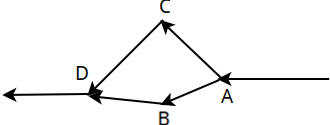
\includegraphics[width=10cm]{pic/anti1.png}
    	   	\caption{蚁群的行为特点}
    	   	\label{fig:anti1}
    	   \end{figure}		   

			信息素会随时间挥发,因而路上的信息素浓度与蚂蚁经过的个数和释放信息素的量
			相关。而蚁群个体根据信息素的浓度,优先选择信息素浓度高的路径。
			
			根据上述蚁群算法写出程序运行后结果如图\ref{fig:anti},总长度为$2946.44724482$。
    	   \begin{figure}[htbp]
    	   	 \centering
    	   	 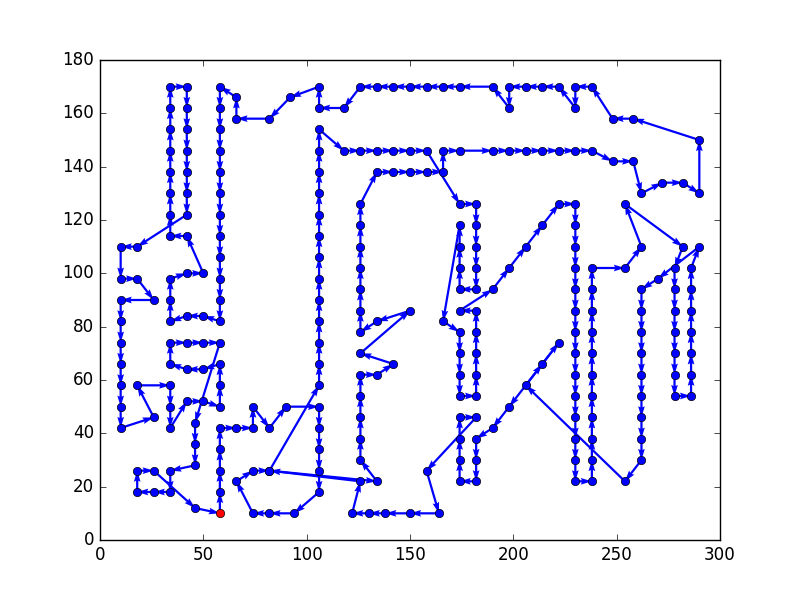
\includegraphics[width=10cm]{pic/anti_result.png}
    	   	 \caption{蚁群算法得到的结果}
    	   	 \label{fig:anti}
    	   \end{figure}
	    	 图\ref{fig:anti}是在迭代次数为2000时的输出图存在多处两个线相互交叉的现
	    	 象,有几处的交叉现象明显的增加了总路径的大小,表明了蚁群算法存在的不足之
	    	 处,进而用遗传算法进行下一步的优化,以便于得到路径更短的输出结果。
      \subsubsection{遗传算法}
      
      遗传算法是模仿生物进化过程的一种算法,它以自然选择和遗传学中的复制、变异和交叉等自然规律为理
      论依据。利用GA算法求解问题,首先需要将模型的解以适当的方式进行编码,并根据模型的目标建立
      个体适应度函数,然后随机生成初始种群(即一组初始的可行解),再重复对种群进行选择、交
      叉、变异等遗传操作直到种群成熟,停止优化\cite{赵静2008数学建模与数学实验}。
      对于NP困难问题智能算法是有效的的选择,我们选用遗传算法对问题一进行建模求解,并且
      根据实际题目的要求对遗传算法进行微调。
        
      %\subsubsection{变异与交叉算子}
      在一般的遗传算法中,种群个体j结构如图\ref{fig:life}所示,变异算子是指让种
      群中某个个体的某些基因突变的算子,
		\begin{figure}[htbp]
			\centering
			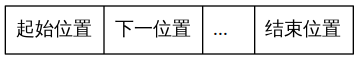
\includegraphics[width=5cm]{pic/life_struct.png}
			\caption{算法中的个体}
			\label{fig:life}
		\end{figure}
        由于本题限定了初始位置与结束位置所以个体基因中的起始位与结束位是固定的
        不可以被突变算子改变,在种群迭代中其过程如如图\ref{fig:cross}所示。
		
        同样的对于算法中的交叉算子,它是使有效基因遗传下
        去的主要算子,在交叉过程中同样应该遵守第一位与最后一位不可算在交叉过程
        中的原则,如图\ref{fig:muate}所示。
        
		\begin{figure}[htbp]
			\centering
			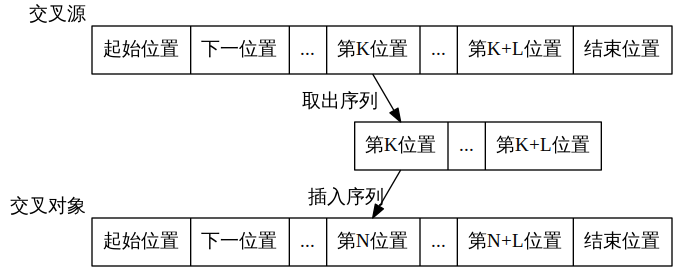
\includegraphics[width=10cm]{pic/life_cross.png}
			\caption{交叉算子}
			\label{fig:cross}
		\end{figure}
		\begin{figure}[htbp]
			\centering
			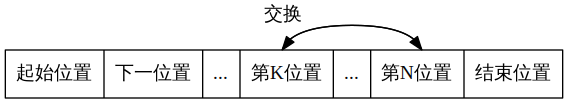
\includegraphics[width=9cm]{pic/life_muate.png}
			\caption{变异算子}
			\label{fig:muate}
		\end{figure}
      %\subsubsection{迭代计算}
        使用上述算法结构对于本问题所给的数据进行种群演化,经过长时间算法运行,得到结果
        如图\ref{fig:ga},总长度为$2775.273329$
        \begin{figure}[!htbp]
        	\centering
        	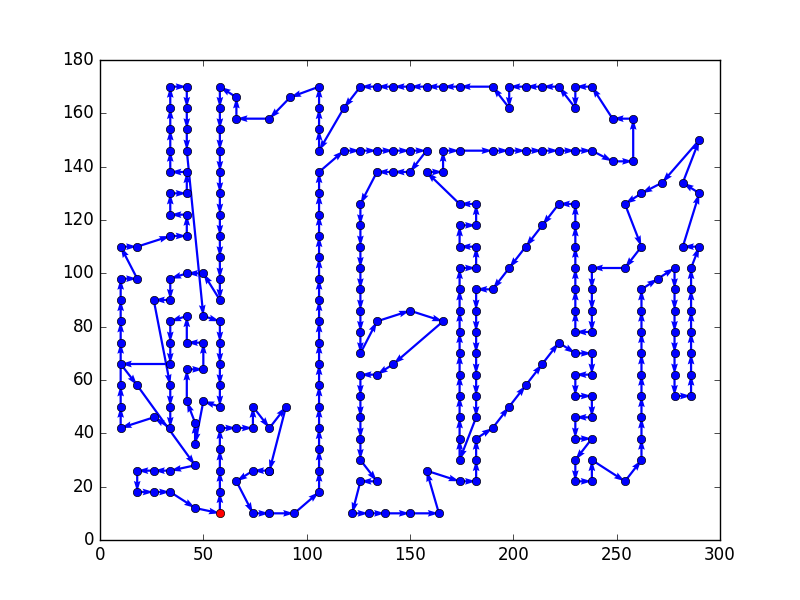
\includegraphics[width=10cm]{pic/ga_result.png}
        	\caption{遗传算法结果}
        	\label{fig:ga}
        \end{figure}
      \subsubsection{改进贪婪算法\cite{饶卫振2012基于求解}}
        贪婪算法是一种构建型启发式算法,其原理是
        求出任意两位点间欧式距离,建立图G的邻接矩阵$D$并为其赋值,其中$d_{i,j}$表
        示位点$x_i$与$x_j$间的距离。将距离矩
        阵中两位点间距离按从小到大的顺序排列,从最短边开始向图$G$中添加,直至添加
        到图$G$成为一条回路为止。
        在添加过程中算法遵循以下原则:
        \begin{enumerate}
        	\item 该节点的链接边数小于2。
        	\item 链接的边不会形成边数小于$n$的回路。
        \end{enumerate}
        
         但贪婪算法在寻找过程中并没有主动使起点与终点回合,所以会造成最后返回路径非常长
         ,如图\ref{fig:fail}所示,这时所得到的总长度为$2861.03928238$。
         \begin{figure}[htbp]
            \centering
            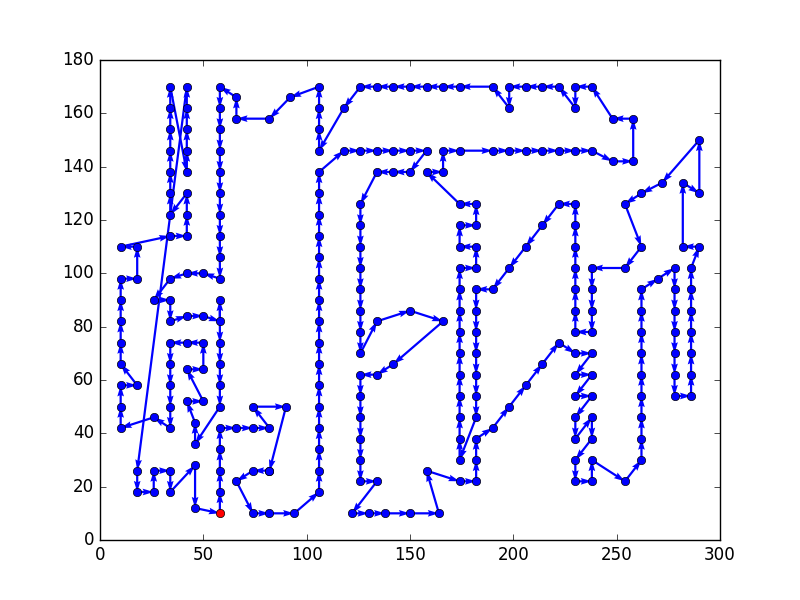
\includegraphics[width=10cm]{pic/greedy_fail.png}
            \caption{贪婪算法得到的结果}
            \label{fig:fail}
        \end{figure}
        分析贪婪算法过程可知,算法最后产生的跨度主要由于算法本身没有确定边的拼接方向,依
        照这种思路对贪婪算法进行改进。
        根据Held与Karp提出的Held-Karp模型\cite{held1970traveling},我们使用一个
        向量$\pi=(\pi_1,\pi_2,\dots,\pi_k)$对
        贪婪算法的距离矩阵$D$进行改造,如式\ref{equ:held-karp}。
        \begin{equation}
	        D'=\left\{
		        \begin{array}{ll}
		        	d_{i,j} = d_{i,j} - \pi_i - \pi_j & \textrm{$i \neq $j}\\
		        	d_{i,j} = M & \textrm{$i=$j}
		        \end{array}
	        \right.
	        \label{equ:held-karp}
        \end{equation}
        其中$M$为一个足够大的数,$\pi_k$由式\ref{equ:pi}构造,其中$\alpha$为比例系数,比例系
        数越大算法就越倾向于先添加外围的点,其中$len_k$是$k$号点到中心的距离,
        $\overline{len}$是所有点到中心距离的平均。
        \begin{equation}
             \left\{
	             \begin{array}{l}
		             \pi=(\pi_1,\pi_2,\dots{,\pi_k}),\pi_k=\alpha\cdot(len_k-\overline{len})\\
		             len_k = \sqrt{(x_0-x_k)^2+(y_0-y_k)^2}\\
		             \overline{len} = \frac{\sum_{k=0}^{k=n}len_k}{n}\\
		             x_0 = \frac{\sum_{k=0}^{k=n}x_k}{n},y_0 = \frac{\sum_{k=0}^{k=n}y_k}{n}
	             \end{array}
             \right.
             \label{equ:pi}
        \end{equation}
        根据改进贪婪算法得到最终结果如图\ref{fig:greedy}所示,总长度为$2791.27883397$。
		\begin{figure}[htbp]
			\centering
			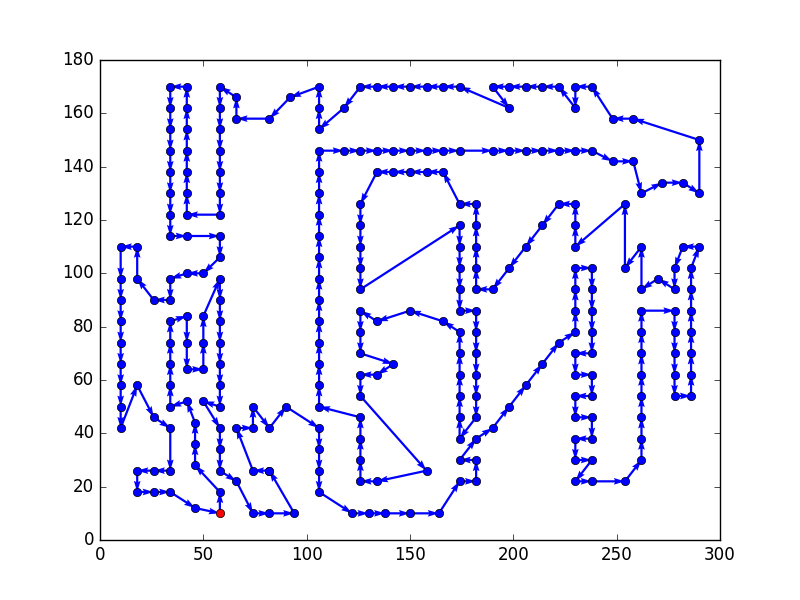
\includegraphics[width=10cm]{pic/greedy_result.png}
			\caption{改进贪婪算法得到的结果}
			\label{fig:greedy}
		\end{figure}

    \subsection{问题二}
	  由于此问不要求起点与终点的位置,而是要求对一万张同样的电路板进行操作,我们
	  采用如下方案进行求解:
	  \begin{enumerate}
	  	\item 求出一个图$G$的解$S$,首尾不需要相接。
	  	\item 从$S$的起点移动到$S$的终点,完成一块电路板。
	  	\item 把上一步的终点作为起点,重复第二步。
	  \end{enumerate}
      \subsubsection{一个链式解}
        遗传算法和蚁群算法可以获得问题的满意解但是其运行过程十分漫长不适用于题
        目要求,所以利用贪婪算法获得链式满意解
        ,如图\ref{fig:greedy2}所示,总长度为$2715.05298165$。
        \begin{figure}[!htbp]
        	\centering
        	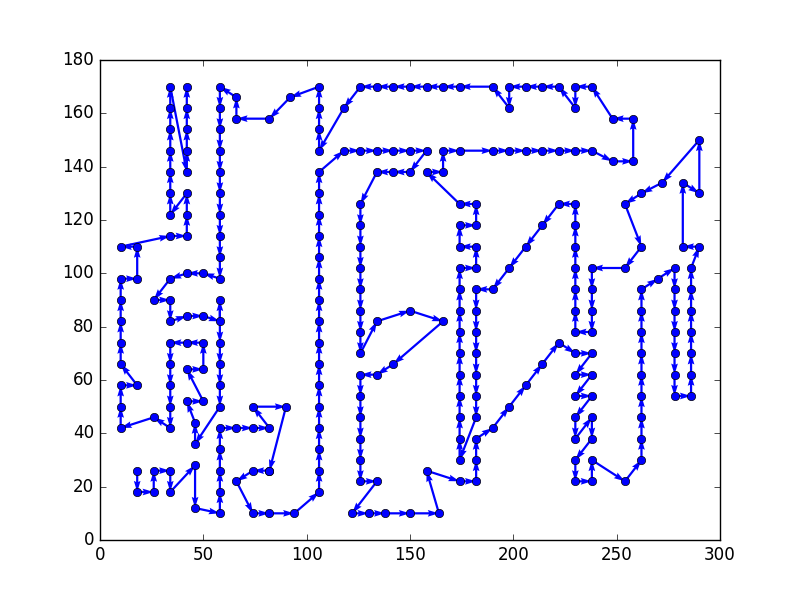
\includegraphics[width=10cm]{pic/greedy_result2.png}
        	\caption{改进贪婪算法得到的结果}
        	\label{fig:greedy2}
        \end{figure}
      \subsubsection{原理}
    \section{模型评价}
  \bibliography{mybib}
  \bibliographystyle{gbt7714}
\end{document}
